% -*-latex-*-
% Document name: approach.tex
% Creator: Rob MacLeod [macleod@cvrti.utah.edu]
%
%%%%%%%%%%%%%%%%%%%%%%%%%%%%%%%%%%%%%%%%%%%%%%%%%%%%%%%%%%%%%%%%%%%%%%
\subsection{Research Approach}
\label{sec:appr}

\subsubsection{Aim 1: Refine an animal model of ischemia to measure electrical potentials within the myocardium, on the heart surface, and on the body surface during controlled ischemic stress }
%\paragraph{Introduction:}
% We will address the lack of adequate
% experimental model to validate electrocardiographic methods
% that characterize and detect acute myocardial ischemia.
We will refine an existing model we have developed
\cite{RSM:Ara2016,BLZ:Zen2018a} that will allow us to record
the electrical activity within the myocardium, on the heart surface, and on
the body surface simultaneously during normal function and with controlled
levels of ischemic stress. A key challenge will be to develop invasive
electrodes that permit closure of the chest cavity. \textbf{Our
  preliminary results suggest we have overcome these and other challenges, and
  thus success in this aim is very likely.} The motivation for
 capturing potentials from all three domains, especially the body surface is
 to increase the translational potential of experimental findings and
 provide a validation dataset to test detection methods.
We will gauge success by our ability to control acute
myocardial ischemia while recording at high spatial and temporal
resolution. The datasets created with this technique would be the first of
their kind and will be shared openly with the research community, enabling
 exciting advances in the study of the electrical response to ischemia, and
 thus understand unique disease mechanisms, improve diagnosis, and validate
 treatment techniques.

\begin{wrapfloat}{figure}{r}{0.5\textwidth}
    % \begin{figure}[htb]
    %     \intextsep{0pt}
    %     \columnsep{3pt}
    \vspace{-.3in}
    \begin{center}
        {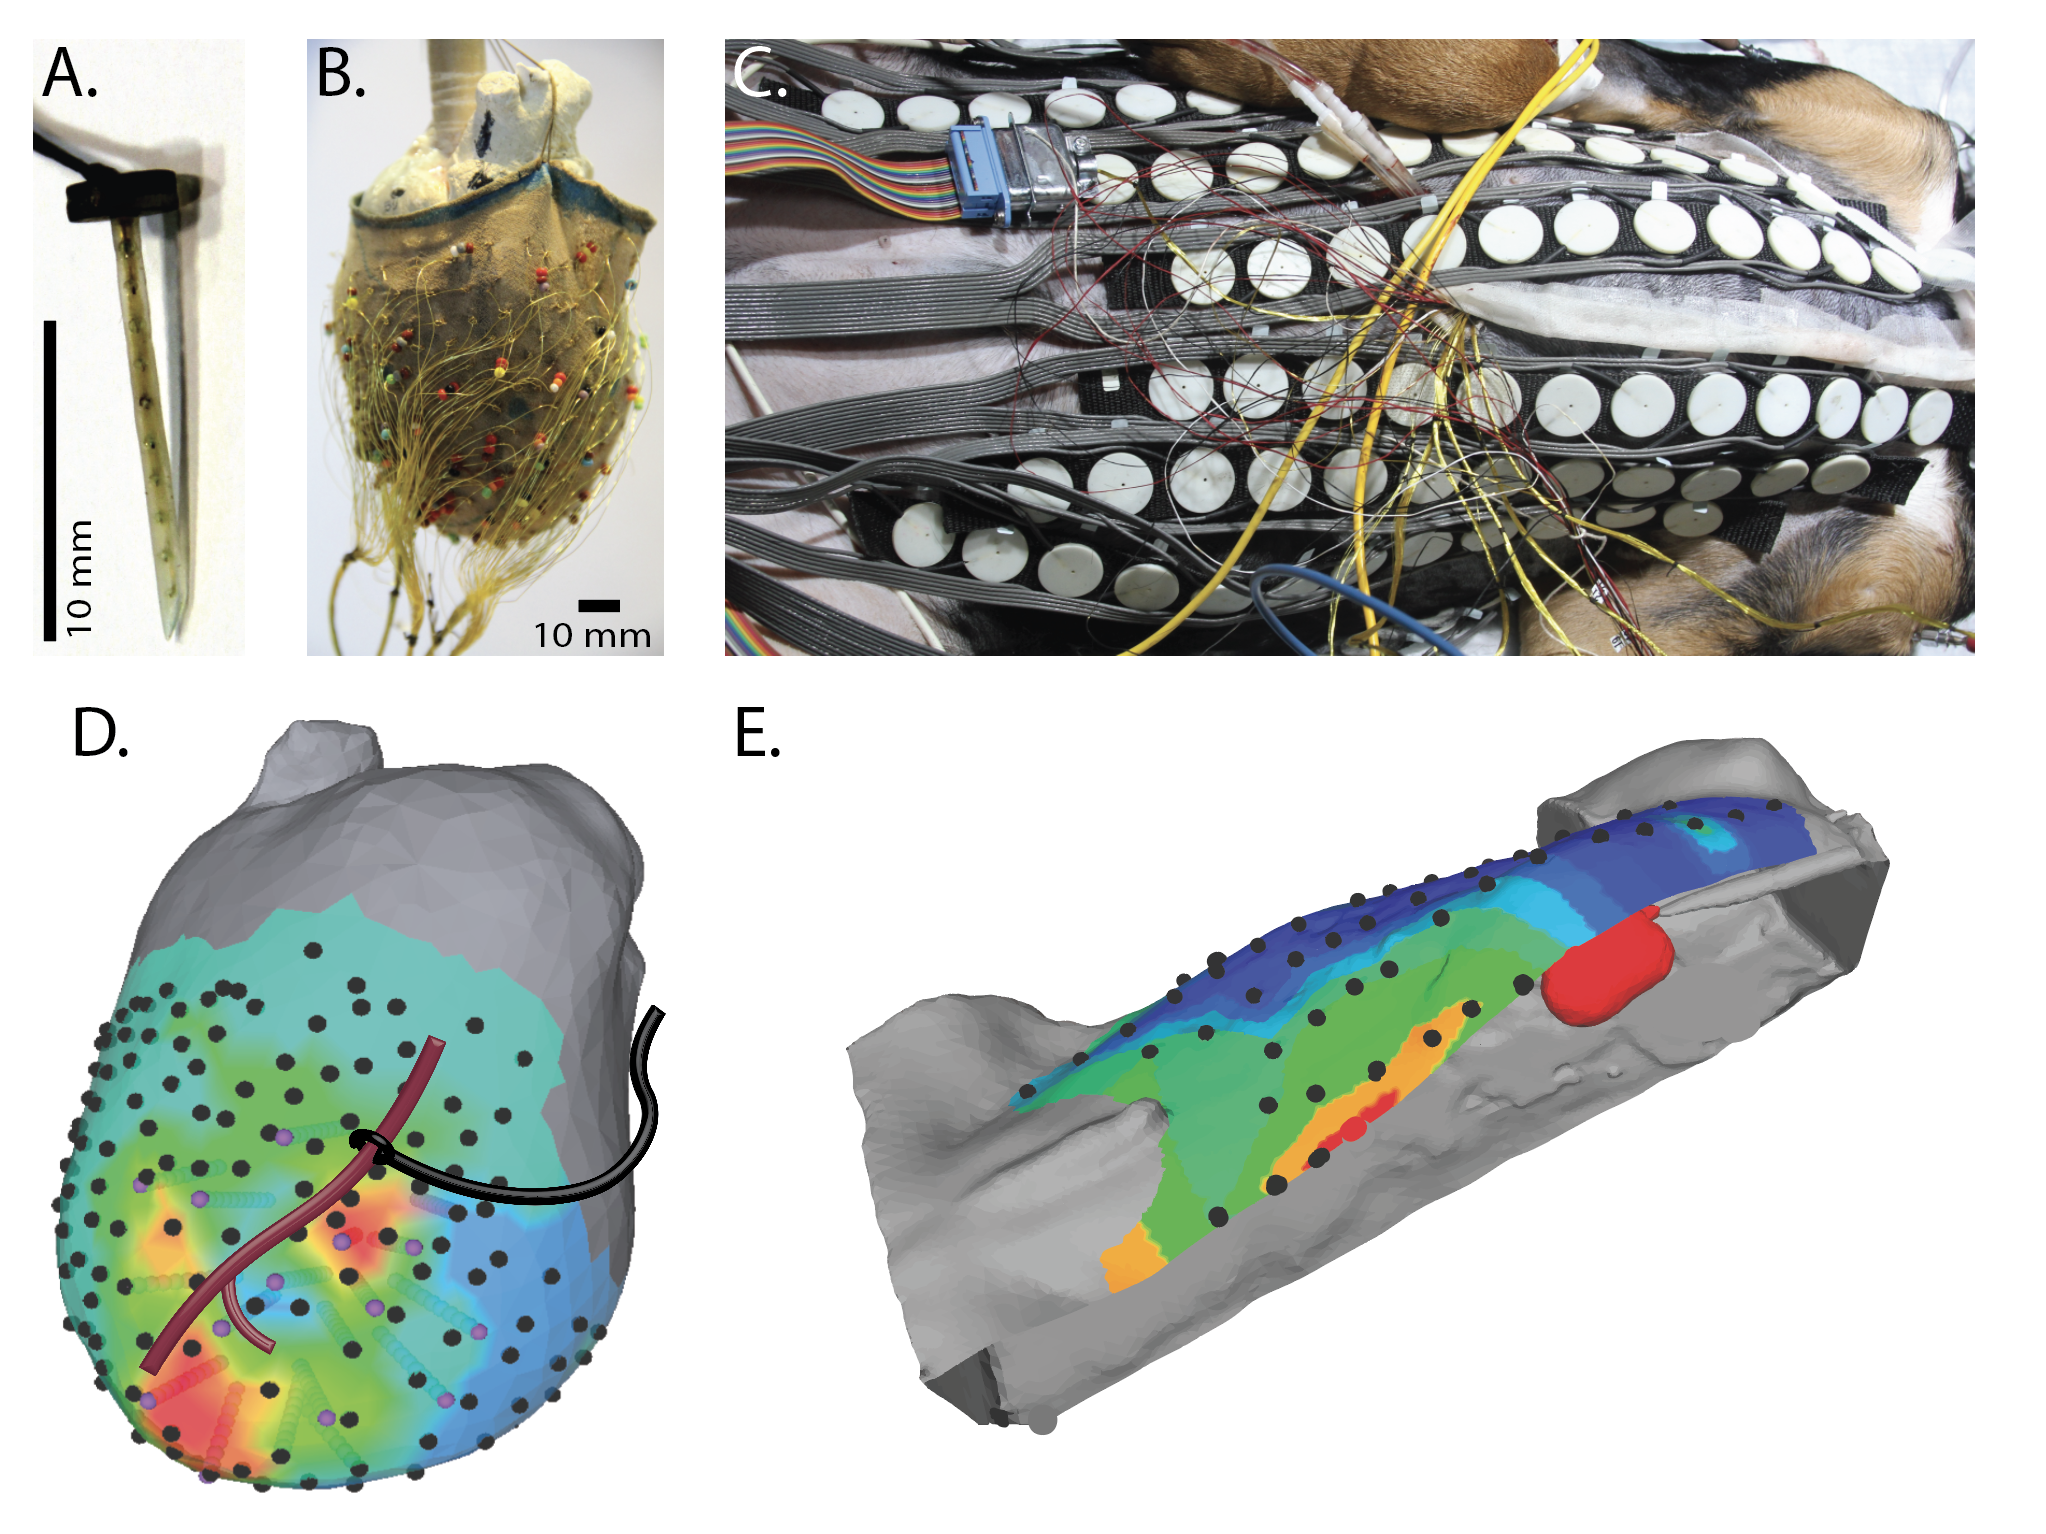
\includegraphics[width=0.5\textwidth]
          {../Figures/fig1.png}}
        \captionsetup{width = 0.5\textwidth}
        \caption{\small \label{fig:prep} Experimental preparation
          components. A. Needle electrode array B. Sock electrode array
          C. Torso surface recordings D. Needle and sock electrodes
          registered on heart geometry with approximate vascular occluder
          location E. Heart and torso surface registered.}
    \end{center}
    \vspace{-.4in}
    % \end{figure}
\end{wrapfloat}

\paragraph{Justification and Feasibility} The justification for this aim
stems from the need for high-resolution electrical recordings of the heart
and body surface under conditions that mimic clinical cardiac stress
testing and simulate acute myocardial ischemia.  Previous studies have
included measurements from fewer than 10 electrodes placed on the heart
surface after occlusion of a major
vessel.\cite{BMB:Hol77a,BMB:Hol77b,BLZ:Kle1978,BLZ:Jan1980} More recent
studies---including from our group---have included measurements from within
the wall.\cite{RSM:Cha89,RSM:Mac95e,RSM:Mac97} These studies
examined the localization and progression of acute ischemia and have
driven a modified clinical paradigm of electrocardiography during ischemia, even
though body-surface ECGs were missing.


The feasibility of the proposed approach lies in our recent progress on an
experimental model that captures the comprehensive electrical response to
acute myocardial
ischemia.\cite{BMB:Ara2009,KKA:Ara2014,RSM:Ara2016,BLZ:Zen2018a} To create
 ischemic stress, we used pacing and a hydraulic occluder around an isolated
 section of the left anterior descending coronary artery. We captured
 electrical potentials within the myocardial wall using 20--30 intramural
 needles, each with 10 electrodes spaced at 1.5~mm along the shaft. A  247-lead sock electrode array provided the simultaneous epicardial
 potentials with spacing of 5~mm.\cite{BMB:Ara2009,KKA:Ara2014,RSM:Ara2016}
With these recordings, we demonstrated that ischemia does not consistently
develop on the endocardial border but in the middle of the myocardial
wall.\cite{RSM:Ara2016}

The feasibility and motivation of our approach are further supported by
progress (including our own) with models that have placed recording
electrodes on the epicardial surface, closed the chest cavity, and then
simultaneously recorded electrical potentials on the body
surface.\cite{BLZ:Spa1975,RSM:Bea2015a,BLZ:Clu2017,BLZ:Zen2018a} These
 studies are sparse in the literature and have lacked the spatial resolution
 and coverage we propose; they have also focused on other pathologies.
 We will refine our existing ischemic model,
 which records potentials from
 the body surface, and apply clinical cardiac stress
 protocols.\cite{BLZ:Zen2018a}
These advancements were enabled with modifications to the manufacturing of
the recording equipment. \textbf{For both aspects, we have preliminary
  results , shown in Figure~\ref{fig:prep} and reported in preliminary
  form.}\cite{BLZ:Zen2018a} In two animal experiments, we closed the chest
following placement of recording and ischemic control equipment. We were
then able to map the electrical potentials during peak ischemic load on the
heart.

% Thus, the experiments proposed here are justified as the only means
% to explore and validate means to diagnose and localize acute ischemia and
% feasible based on previous results from the literature and our group.




\paragraph{Experimental Design} \textit{Technical goal 1: To obtain ischemic load
  control.} To create cardiac stress, we will modify regional perfusion and
myocardial stress independently. To decrease the perfusion, we will place a
calibrated hydraulic vascular occluder (Precision Technologies) around the
left anterior descending coronary artery of a canine or swine. The occluder will vary the
perfusion percentage in fine steps (5\%) and provide a full range of flow
(100--0\% of normal). To increase myocardial stress, we will increase heart
rate with either electrical pacing via a right atrial pacing clip, or
pharmacological stress via beta-1 adrenergic stimulation from
dobutamine. We will induce 5--20-minute episodes of ischemia and vary the
occlusion percentage from 50\%--90\%, the pacing rate from 100--250 beats
per minute, and the dobutamine infusions from 5--40
$\mu$grams/kg/min.\cite{BLZ:Man1988} Following each episode, the heart will
rest for 30 minutes and return to baseline electric potentials, after which
we will capture control recordings. To test if cardiac ischemia was
induced, we will visualize ST40\% potential values from continuous
recordings before, during, and after each ischemic episode. Each animal
will serve as its own control and will have several replicates of identical
ischemic protocols to ensure accurate and consistent data.
% For this
% technical goal, we expect to have complete control of the metabolic supply
% and demand of the heart during an ischemic episode.

\textit{Technical goal 2: To simultaneously record epicardial and
  transmural electric potentials from the myocardium.} To record epicardial
potentials, we will create an electrode array with 247 evenly distribute
silver wires around the epicardial surface of the ventricles. To record
intramural potentials, we have designed plunge-needle electrodes that
evenly sample the myocardial wall at 1.2 mm spacing. For each
experiment, one epicardial electrode sock and 20--30 intramural needles
will record electrograms from the healthy and ischemic regions. After
placing the electrodes within and around the heart, we will tunnel each
cable through a transthoracic opening and wire, suture and glue the chest to
minimize air leaks and reestablish an intact thorax. After the chest
closure, approximately 70--120 body-surface electrodes mounted in vertical
strips (depending on animal size) will be attached to the skin.

Signal acquisition will occur with an existing custom multiplexer capable
of sampling up to 1024 channels at 1~kHz frequency.   Following each experiment, the electrode locations will be
identified via MRI imaging and other validated registration
techniques.\cite{BLZ:Zen2018a} All resulting electrograms will be processed
using our custom, open-source software.\cite{RSM:Rod2018}


\paragraph{Expected Results} We expect to achieve an experimental model in
which we can reproducibly control the ischemic stress on the heart and
simultaneously record myocardial electrical potentials from within the
myocardium in and around the perfusion bed affected by
occlusion, 360-degree coverage of the epicardial surface, and on the body surface.  For this
model to be considered valid, it must induce transient episodes of
myocardial ischemia within the heart, returning to baseline electric
recordings within 30 minutes after an intervention. The spatial sampling
must be adequate to discern ischemic zones within the myocardium. From our
experience, the minimum amount of ischemia required to alter signals on the
epicardial surface of the heart is roughly 5 mm diameter spheroid
shapes. Thus, we require resolution at half that size (2.5~mm).  The signal-to-noise ratio must be over 10:1. The combination of these metrics would confirm that the experimental model is accurately recording and controlling transient myocardial ischemia.

To control for potential confounding variables between experiments we will perform ``normalization'' interventions at the beginning of each experiment. These interventions will have a set heart rate and occlusion percentage that is used consistently at the beginning of each experiment. This will provide an indication of the relative differences between each experimental model and if the results can be directly comparable between each model. 
%%%% Enlarge here


\paragraph{Potential Problems and Alternative Strategies} The first
possible hurdle is achieving a tight seal along the chest incision and
minimal residual air in the chest.  Should either situation arise, we will
explore different closure materials under guidance from our surgery
colleagues. To remove excess air, we will apply vacuum suction through
chest tubes. Another general concern is the stability of the animal
model. Measures we will explore include implementing a fluid management
system and an antiarrhythmic drug regimen; tracking the stability using
blood gas values, blood pressure, ${\rm pCO_2}$, oxygen saturation, and
blood pH; and reducing the number of needle electrodes.


%%%% Enlarge Here

\subsubsection{Aim 2: Test the hypothesis that exercise and dobutamine infusion create identical regions of myocardial ischemia}

 Currently, there is no definitive evidence to compare ischemic zones with
 different heart stressing mechanisms.
In this aim we will test the
hypothesis that the electrocardiographic response to ischemia has similar
features during exercise and dobutamine stress. The approach is to use our
experimental model
 with high-resolution electrical recordings and
 controlled ischemia
to characterize the ischemic zones created by each
stress mechanism. 

\paragraph{Justification and Feasibility} The justification for this aim
is that any differences in the response to these two commonly used forms of
cardiac stress should be reflected in the ECG-based metrics and thresholds
used in clinical testing.  Despite the assumed similarities between exercise
and pharmacological (typically dobutamine) stress, we will be the first to
our knowledge to examine the extent, location, or electrocardiographic
profile at high resolution of ischemia produced by these two
modes. \textbf{Our preliminary results have shown a small difference in the
  regions of ischemia produced by each stress mechanism, shown in
  Figure~\ref{fig:dobutvspacing}.}

 We will employ two clinical methods
 to induce cardiac stress when detecting myocardial ischemia. The first
 method requires the patient to exercise at a set level and steadily
 increase the exercise rate at set intervals.\cite{BLZ:Oki1986} The most
 common exercise protocol is the Bruce stress test protocol, which has five
 exercise stages, with each stage lasting 3
 minutes.\cite{BLZ:GOL1976,BLZ:Bru1963,BLZ:Oki1986} If a patient is unable
 to exercise, a pharmacological stress test with dobutamine can be
 used.\cite{BLZ:SAL1992,BLZ:Gre1997,BLZ:Man1988} Dobutamine is primarily a
 beta 1 agonist which increases heart rate and contractility and simulates
 exercise. 

Several studies have demonstrated differences in performance between
exercise and dobutamine stress tests using a variety of markers.  From an anatomical point of view, the ischemic
zones created should not be different. However, with complex physiology,
possible drug binding to other receptors, and many other confounding
factors, the possibility for differences cannot be ruled out. If the
ischemic zones created are different, ischemia detection methods may have
to be tailored to the cardiac stress type, or at the very least, physicians
should be informed of the possible differences between the ischemic zones
created by each mechanism.  

\paragraph{Experimental Design} Using the experimental system described
above, we will compare rapid pacing (simulating exercise) and dobutamine infusion for their
ability to create ischemia. Our proof of concept results suggest we can
carry out both stresses in the same animal and that they may produce
different results.  To simulate exercise stress, we will first determine
the resting heart rate and apply stepwise increase as per the Bruce
exercise stress protocol (6--8 steps at 3-minute
duration).\cite{BLZ:Oki1986} Pharmacological stress will occur by infusions
at 5--40 ug/kg/min per the dobutamine protocol (6--8 steps at 3-minute
duration).\cite{BLZ:SAL1992} Recovery between repeated episodes will last
30 minutes. Vascular occlusion will be held constant for each
intervention. To reduce order dependencies, we will vary the pattern of
interventions. We will compare relative differences between ischemic zones induced within experiments to control for vasculature and other physiological variability.


\begin{figure}[htb]%{\textwidth}
    % \begin{figure}[htb]
    \vspace{-.3in}
    \begin{center}
        {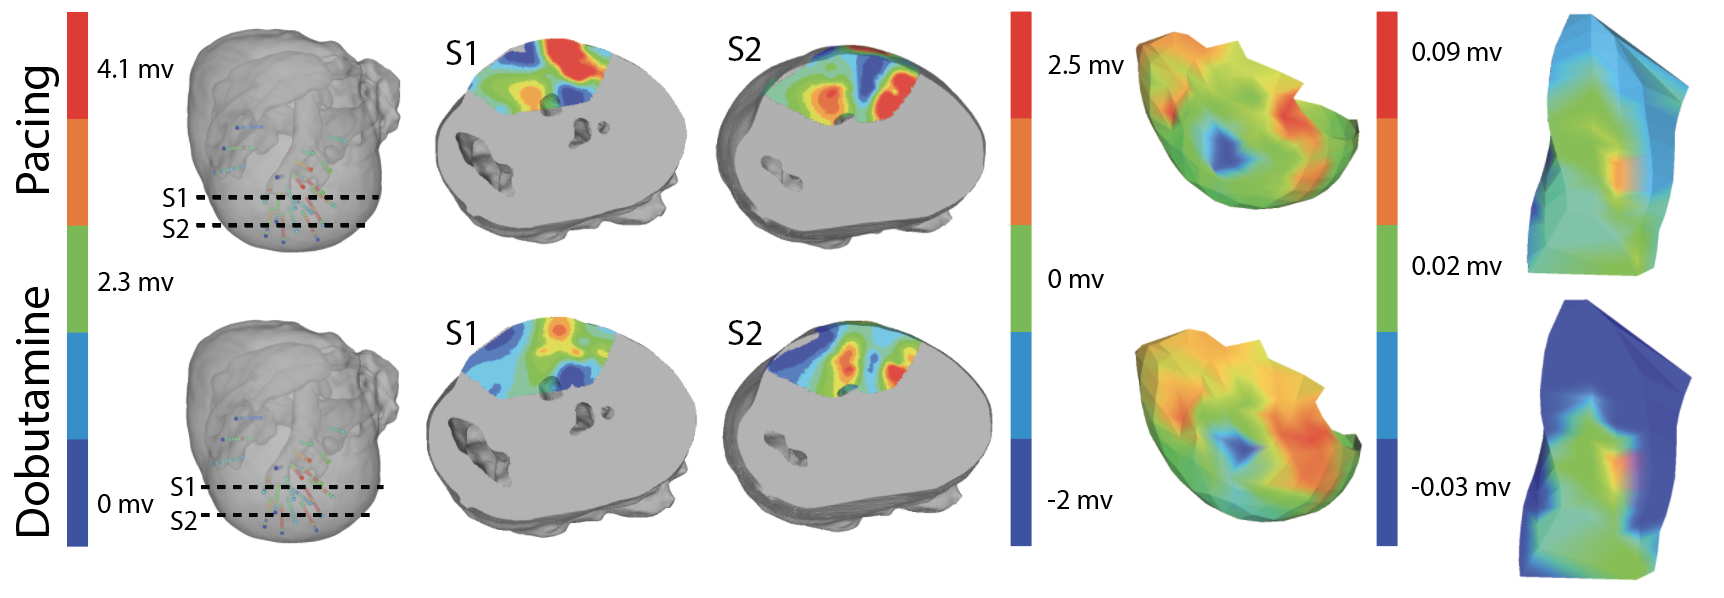
\includegraphics[width=\textwidth]
          {../Figures/fig2.png}}
        \captionsetup{width = \textwidth}
        \caption{\small \label{fig:dobutvspacing} Images of the
          intramural, epicardial surface, and torso surface recordings
          during peak ischemia for dobutamine and pacing protocols.}
    \end{center}
    \vspace{-.25in}
    % \end{figure}
\end{figure}


Data analysis will consist of comparing the extent and the characteristics
of the ischemic regions over time that arise from these two different
stress interventions. First, the ST40\% value across the entire region of
perfusion will be compared using Pearson's correlation coefficient and
relative error approximations. Next, thresholds to the ST40\% values
measured will be applied at multiple time points within the ischemic
intervention, which will create distinct volumes of ischemia. Both the
three-dimensional volume and location of the ischemic zones will be
compared using Dice overlap coefficients and statistical shape analysis.

\paragraph{Expected Results} Based in preliminary results, we expect some
variation to arise between the two stress mechanisms.  We will use the Dice
coefficient to test our null hypothesis (greater than 80\% overlap), and
compare the raw values of ST40\% via Pearson's correlation
coefficient above 0.80. Agreement in both of these metrics would
substantiate the hypothesis that the ischemic region created during
different stress tests is identical. With identical occlusion amounts and
locations along the coronary vasculature, the two regions of ischemia
should be the same. 

To limit the possible confounding factor of the order of each intervention within an experiment we will vary the intervention order per experiment, \ie{} start with a dobutamine stress protocol then a bruce stress protocol in one experiment vica versa in the next experiment. 

The experimental results will be interpreted as ...... 


\paragraph{Potential Problems and Alternative Strategies} This study is
focused on ST-segment shifts as the basis for ischemia determination, but
we will explore other reported metrics in the electrogram signal, which
include the end of the QRS, peak of the T wave, or peak-to-peak amplitude
of the QRS. Another potential problem is adverse reactions to dobutamine
infusion in the animal, for which we would substitute other drugs with
similar influences, such as isoproterenol to increase heart rate alone,
arbutamine to increase heart rate and contractility, or other similar
beta-1 agonist or cardiac stimulants.

\subsubsection{Aim 3: Test the hypothesis that ECG imaging techniques can be used to detect and localize ischemic regions within the heart}

The objective of this aim is to develop and apply a novel ECGI approach to
localize and detect ischemic sources within the heart. We will use our
expertise in ECGI techniques in conjunction with our refined experimental
models. Success in this aim will impact clinical care of a very common
condition by creating a new, highly sensitive and specific test to detect
myocardial ischemia noninvasively.

\paragraph{Justification and Feasibility}
 ECGI is an emergent technology that
 is used to detect the source of the electrical signals within the heart
 from body-surface recordings.
ECGI has been applied to several different pathologies at multiple centers
and has developed into commercial products. Current techniques have focused
on isolating the locations of premature ventricular contractions (PVCs), atrial
fibrillation, T-wave alternans, repolarization gradients, and other
conditions.\cite{BLZ:Pot2014,BLZ:Dub2015,BLZ:Wan2016a,RSM:Sha2015,BLZ:Wan2018}
The results from these techniques have shown promise to further the
technology and increase the applicability to other conditions.

Our study will be the first of its kind to attempt to create and to
validate an ECGI reconstruction approach that achieves millimeter and
millisecond resolutions of regions of ischemia within the heart. Our newly
developed experimental model and long-established expertise in ECGI place
provide a substantial advantage to further these goals and create a system
with a large clinical impact.


\paragraph{Experimental Design} ECGI is an image reconstruction technique in
which each electrode lead is a projection of the sources of bioelectricity
within the heart onto the body-surface.\cite{RSM:Mes86,RSM:Pul2010} The
goal of ECGI is then to combine all these projections and
\emph{reconstruct} the electrical sources within the heart. As with
conventional medical imaging modalities, the mathematical formulation of
ECGI requires both a forward model and an inverse reconstruction
approach. The forward model describes the relationship between the assumed
known electrical activity within the heart and the body-surface potentials
and captures the influence of torso geometry and electrical
conductivity.\cite{RSM:Mac2010b} The inverse problem is based on the
forward model but seeks to invert or reconstruct it, a simple concept with
many practical challenges.  The inverse problem is also the more relevant
as it assumes no knowledge of the sources in the heart but rather of the
measured body-surface potentials and seeks to determine the cardiac
sources.\cite{RSM:Mes86,RSM:Pul2010}

A forward model consists of three parts, the cardiac source, the model
output (in this case body surface potential recordings), and the volume
conductor. The cardiac source can be represented by several different
quantities such as an extracellular potential measurement or transmembrane
potential (TMP) measurement. Selecting which source to use for specific
applications is an important because the source approximation must show
significant changes in the metric you are attempting to detect. The forward
solution incorporates all three parts (the source, output, and volume
conductor) to determine the relationship between the electrical source and
the measured output using the individual volume conductor and electrical
conductivities unique to each patient, which creates accurate and patient
specific source localizations.

An inverse model is simply the forward model in reverse. To implement an inverse model several initial
assumptions must be made, which are: the problem is quasistatic, no current
flows across the torso surface, and only extracellular current flows into
the torso. If we assume that
the forward model is a good approximation of the patient and conductivities
of the volume conductor then a simple inversion of the system should
provide an accurate solution of the cardiac source. However, the inverse
problem in electrocardiography is inherently il-posed because small
fluctuations in the recorded signal produce unbounded fluctuations in the
cardiac source representations. This means the inverse model of
electrocardiography is highly susceptible to noise from body surface
recordings, geometric model locations, and electrode registration causing
large perturbations in the solution. To minimize the effect of noise, we
apply multiple constraints and optimize the solution to realistic
physiological values. The constraints can be modified, adjusted, or
removed based on the unique electrical source. The solution is then fit to
the constraints via a variety of possible optimization methods. Both the
constraints and optimization method applied can be customized to fit the
specific problem being solved.


The main design choices in implementing ECGI, \ie{} of solving this inverse
problem, include the particular representation of the cardiac sources, the
level of detail in the geometric model of the thorax, and the means by
which to apply necessary constraints to the reconstruction of cardiac
sources from measured body-surface potentials.  Constraints are
needed---just as with all image reconstructions---to deal with the
physically ill-posed nature of the resulting inverse problem. A problem
that is ill-posed responds to even small fluctuations in the input data
with nonlinear, unbounded fluctuations in the outputs, in our case the
cardiac source representations. This response means the inverse problem of
electrocardiography is highly susceptible to noise from, \eg{} body-surface
recordings, geometric model approximations, or electrode registration
errors. To minimize the effects of noise, we apply multiple constraints and
optimize the solution to reflect realistic physiological values.

For this application, we will construct an ECGI solution based on the
source model of transmembrane potentials (TMPs) throughout the ventricles
and imposing realistic physiological constraints on their reconstruction
using what is known as a ``total variation optimization technique'', which
we have shown previously to be a feasible approach for this
application. \cite{RSM:Wan2011b,RSM:Wan2013} We will both expand on these
initial results, for example by evaluating a wide range of constraints, and
also drive their implementation and validation with detailed experimental
data from the other aims of this research. This model is an ideal
validation source because it is capable of locating ischemic regions,
generating precise geometric models of the thorax, and placing the
recording electrodes with millimeter accuracy. 

A key numerical challenge of this approach is how to compare predicted
reconstructions with measured data and then use these insights to set the
weights of various constraints in the optimization technique.  We will use
a combination of qualitative comparisons extracted from visualizing the
results and a set of statistical metrics. These metrics will include
Pearson's correlation coefficient and root-mean-squared and relative errors
along with absolute maximal errors.  In addition, we will use thresholds of
ischemic TMP values to determine the volume, shape, and location of
ischemic zones, measured by the Dice overlap coefficient.

\paragraph{Expected Results} We must achieve several specific results for
this ECGI approach to serve as a viable method to detect ischemia. First,
the method must reproducibly detect ischemic regions down to regions
equivalent to a sphere of 5~mm diameter. This threshold is derived from our
previous measurements of the smallest possible ischemic region that creates
changes in epicardial potentials.  We will also require correlations above
0.80 and relative errors below 10\%. These metrics indicate that the
measured and simulated electrical potentials are highly similar. Finally,
to ensure accurate localization of ischemia, we expect a Dice overlap
coefficient to be above 0.80. Such accuracy would indicate that the
thresholded regions of ischemia detected are sufficiently similar. The
combination of these results would support the hypothesis that ECGI can be
used to detect acute myocardial ischemia from body-surface
potentials. Deviation in any one of these results would substantiate
further investigation and refinement of the ECGI techniques to better
localize and detect the ischemic sources within the myocardium.

%%% Enlarge Here

\paragraph{Potential Problems and Alternative Strategies} Applying ECGI
includes many design and parameter choices, which provide both challenges
and a wide range of alternative strategies. The most basic choice is the
source of cardiac bioelectricity, which we could adjust from transmembrane
to extracellular potentials, an approached used in the past by us and
others with known strengths and weaknesses \cite{RSM:Mac95,RSM:Ost97b}. We
could also increase the number and nature of the constraints to force known
shapes and textures of ischemic sources. However, increasing the number of
constraints introduces more inherent bias toward a particular solution,
which, in turn, may produce misleading ischemic sources. Other mathematical
optimization methods could also be used for this
application\cite{RSM:Ahm94,RSM:Bro96b,RSM:Ahm98,
  RSM:Gha2001,RSM:Ost92,RSM:Ost97c,RSM:Ram2003,RSM:Clu2018}.

%%%% Enlarge Here

%
%%\begin{wrapfigure}[25]{r}{0.6\textwidth}
%\begin{figure}[htb]
%	\vspace{-.1in}
%	\begin{center}
%		{\includegraphics[width=0.6\textwidth]
%			{Figures/block-diagram.pdf}}
%		\caption{\small \label{fig:block-diagram} Block diagram of the
%			proposed MRI guided ablation system.  Numbers in each block
%			indicate the associated specific aim.}
%	\end{center}
%\end{figure}
%%\end{wrapfigure}
%
%Figure~\ref{fig:block-diagram} summarizes the steps involved in carrying
%out the proposed research.  Other have described the details of this
%organization~\cite{RSM:Ver2011,RSM:Vij2010} and we will build on these
%ideas with the goal to refine the accuracy and improve the robustness of
%the system. 
%
%
%% This structure also shows the alternative list structures in action. 
%% Their goal is to reduce the space required. 
%\begin{desclist}
%  \item[Year 1:] \mbox{}
%    \begin{numlist}
%      \item 
%      \item 
%      \item 
%    \end{numlist}
%  \item[Year 2:] \mbox{}
%    \begin{numlist}
%      \item 
%      \item 
%    \end{numlist}
%  \item[Year 3:] \mbox{}
%    \begin{numlist}
%      \item 
%      \item 
%    \end{numlist}
%  \item[Year 4:] \mbox{}
%    \begin{numlist}
%      \item 
%      \item 
%    \end{numlist}
%\end{desclist}